\subsubsection*{Training Insights}
Not a single ResNet152 training managed to produce a model that is able to predict with a $\sigma < 2$. In combination with the long training times (see \autoref{tab:model_params}), this makes ResNet152 the least efficient ResNet model. Many models were not able to keep the predictions within the correct mass range and thus three trainings reached $\sigma$ values of over $10^4$.

\begin{figure}[H]
\centering
\begin{subfigure}{.46\textwidth}
\centering
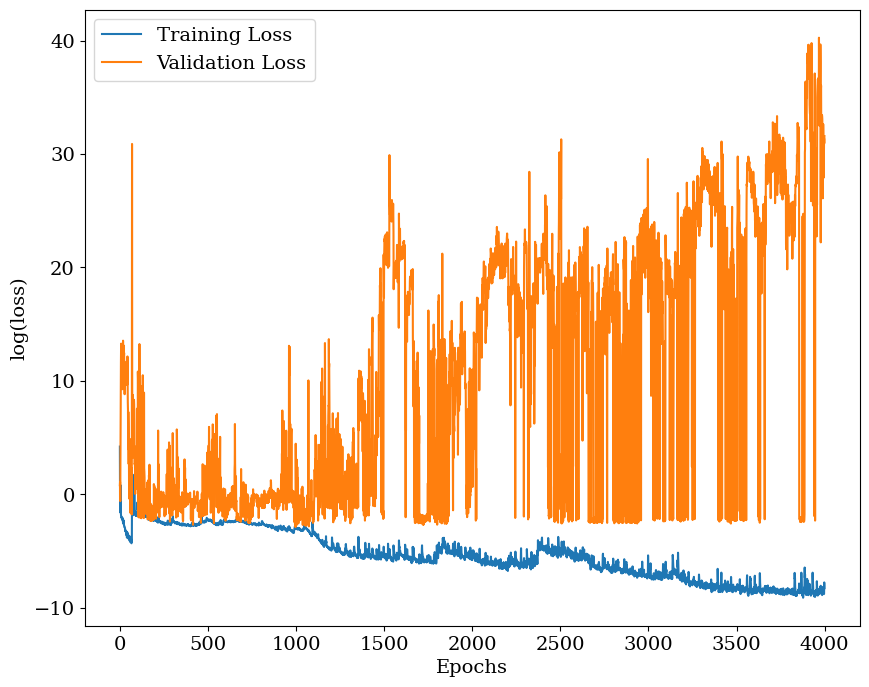
\includegraphics[width=\textwidth]{images/Chapter4/Res152/res152_bad_1.png}
\caption{} 
\label{fig:res152_bad_a}
\end{subfigure}
\hspace{.6em}
\begin{subfigure}{.46\textwidth}
\centering
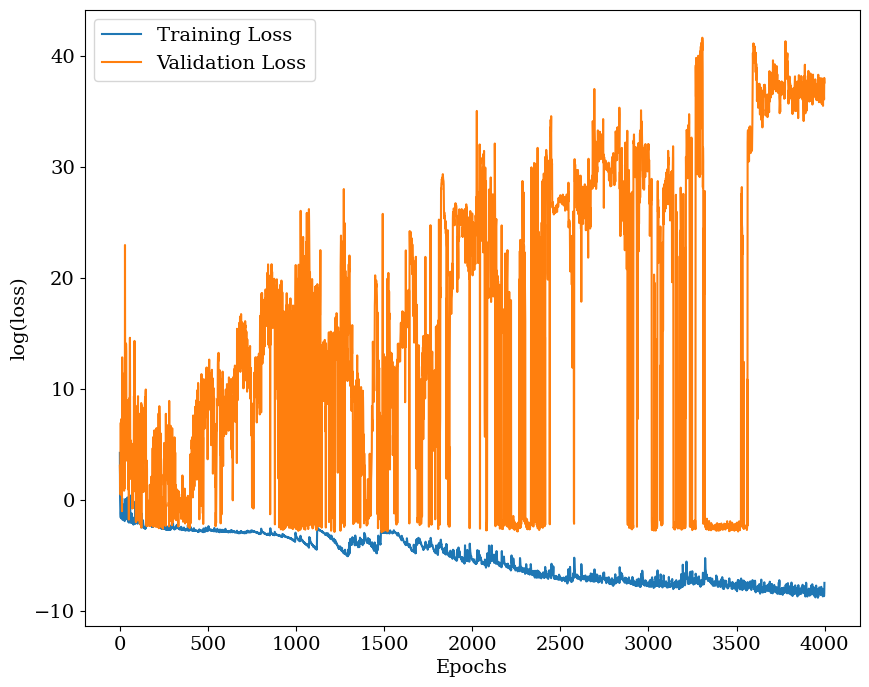
\includegraphics[width=\textwidth]{images/Chapter4/Res152/res152_bad_2.png}
\caption{} 
\label{fig:res152_bad_b}
\end{subfigure}
\caption{Two of the three very bad trainings of ResNet152. Validation loss kept on spiking up at many epochs. In \autoref{fig:res152_bad_b}, validation loss was steadily low for a few hundred epochs but spiked up again before the end of training.}
\label{fig:res152_bad}
\end{figure}


\subsubsection*{Best Performing Model}
The best ResNet152 model did not suffer from the spikes seen in \autoref{fig:res152_bad}. Nevertheless, predictions are not that accurate compared to the other models and considering the lower $\sigma$ at the training predictions, overfitting might be the cause of this.


\begin{figure}[H]
\centering
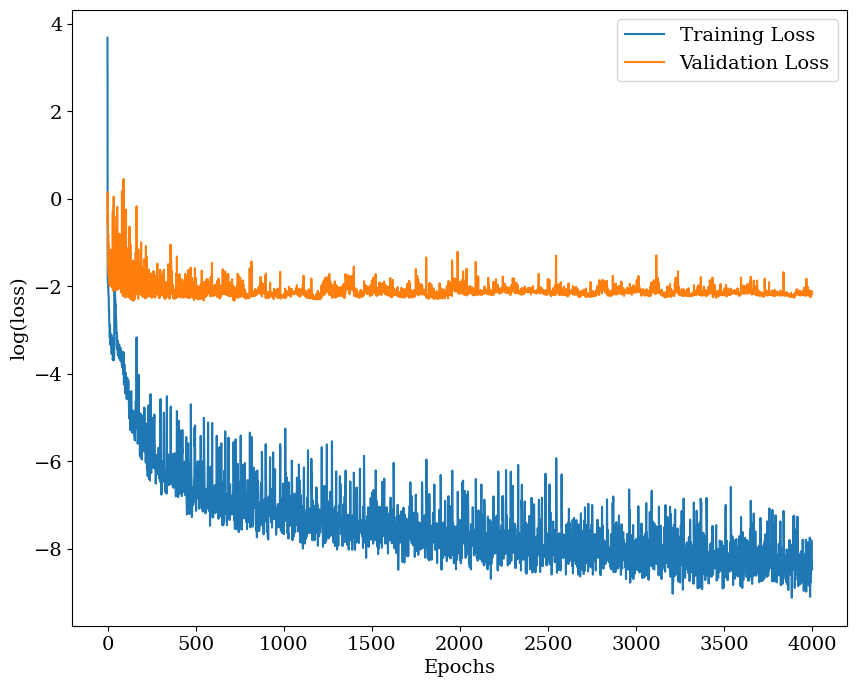
\includegraphics[width=.667\textwidth]{images/Chapter4/Res152/res152_history.png}
\caption{Training history of the best performing ResNet152 model.} 
\label{fig:resnet152_best_history}
\end{figure}

As seen in multiple other ResNet trainings, the model tends to estimate smaller galaxy clusters ($\log{(M_{500}^{\text{true}}/M_{\odot})} < 14$) too high and bigger galaxy clusters ($\log{(M_{500}^{\text{true}}/M_{\odot})} > 14$) too low. This feature can be seen in both the training and the test predictions. As a result of this, the overall $\mu$ value is close to zero.


\begin{figure}[H]
\centering
\begin{subfigure}{.46\textwidth}
  \centering
  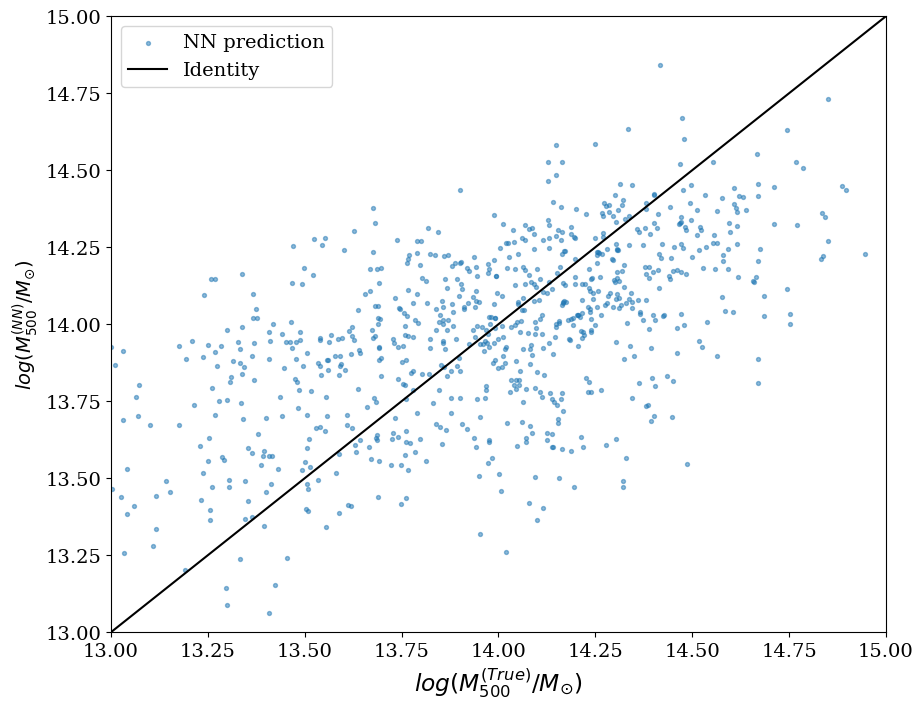
\includegraphics[width=\linewidth]{images/Chapter4/Res152/res152_test.png}
  \caption{Model predictions on the test set.}
  \label{fig:best_perf_resnet152_a}
\end{subfigure}%
\hspace{.6em}
\begin{subfigure}{.46\textwidth}
  \centering
  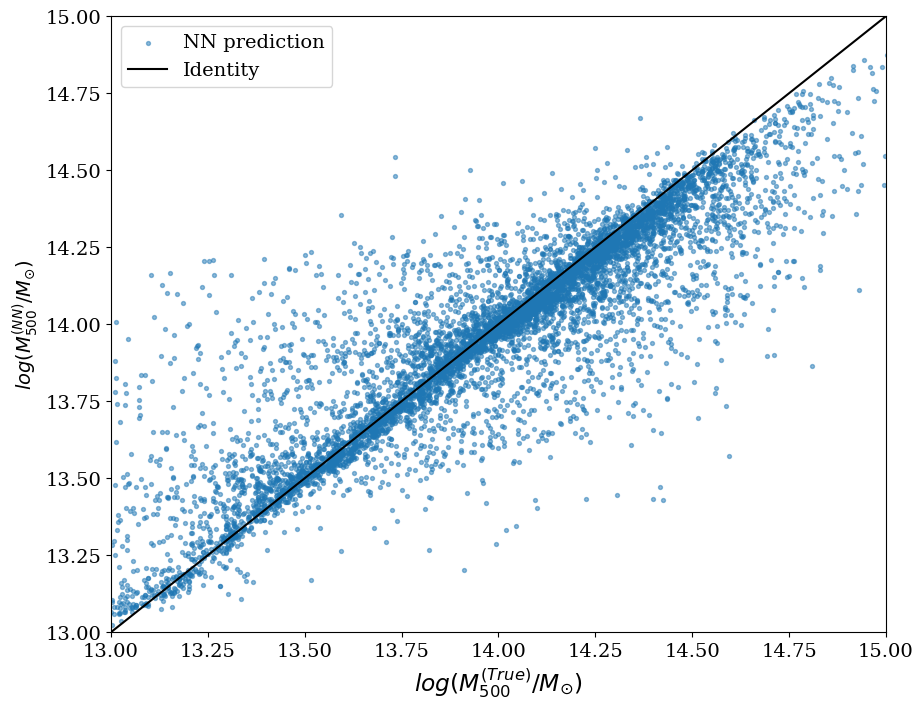
\includegraphics[width=\linewidth]{images/Chapter4/Res152/res152_train.png}
  \caption{Model predictions on the training set.}
  \label{fig:best_perf_resnet152_b}
\end{subfigure}
\begin{subfigure}{.46\textwidth}
  \centering
  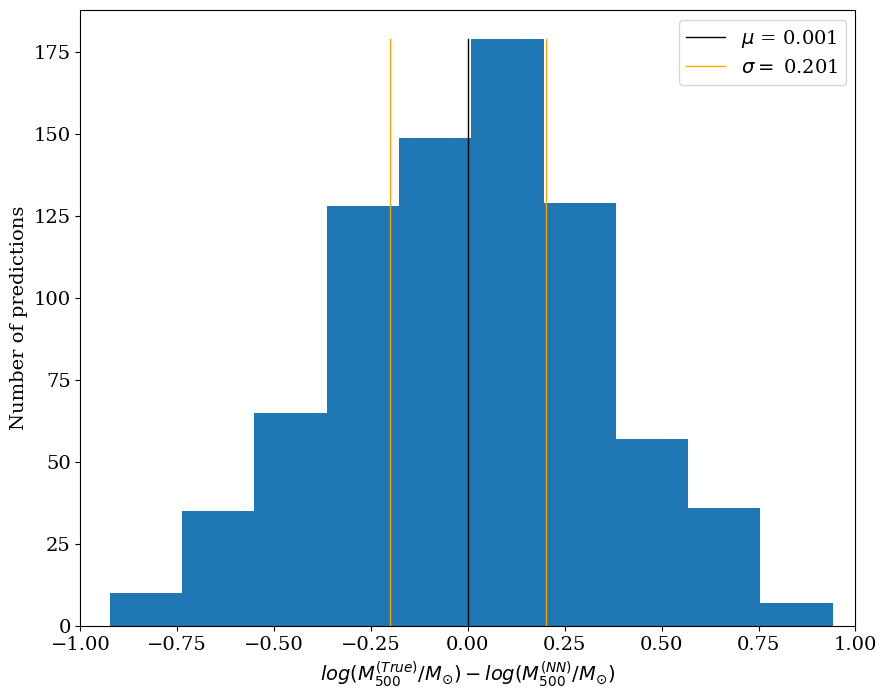
\includegraphics[width=\linewidth]{images/Chapter4/Res152/res152_test_hist.png}
  \caption{Histogram of model predictions on the test set.}
  \label{fig:best_perf_resnet152_c}
\end{subfigure}%
\hspace{.6em}
\begin{subfigure}{.46\textwidth}
  \centering
  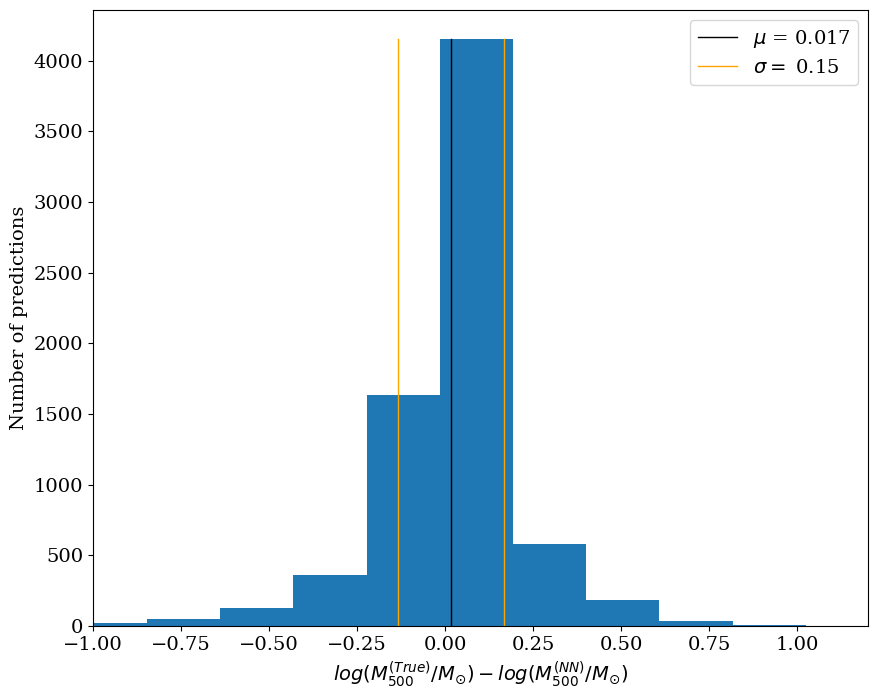
\includegraphics[width=\linewidth]{images/Chapter4/Res152/res152_train_hist.png}
  \caption{Histogram of model predictions on the training set.}
  \label{fig:best_perf_resnet152_d}
\end{subfigure}
\caption{ResNet152 training results are worse than all the other ResNet models trained. The better training predictions could be explained by overfitting.} 
\label{fig:best_perf_resnet152}
\end{figure}